\section*{Лекція 1: Знайомство з Python}
 
\subsection{Вступ}
\begin{frame}
\frametitle{Викладач}
\begin{wrapfigure}{r}{0.35\textwidth}
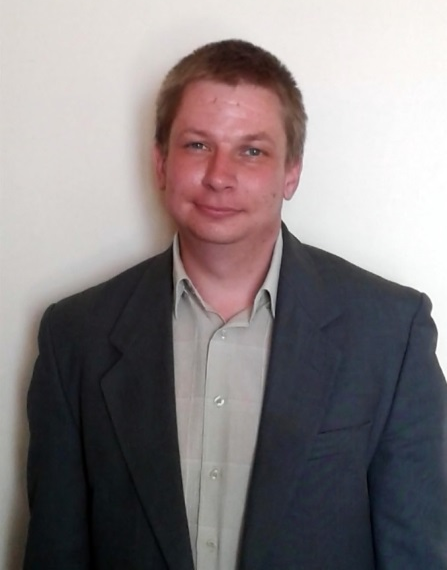
\includegraphics[width=0.2\textwidth]{pictures/myphoto}
\caption{Легенький М.М.}
\label{myphoto}
\end{wrapfigure}
\textbf{Легенький Максим Миколайович}

доцент кафедри теоретичної радіофізики

\textit{факультету радіофізики, біомедичної електроніки та комп’ютерних систем}

aуд. 5-5

тел. (057) 707-52-57

e-mail: \href{mailto:mlegenkiy@karazin.ua}{mlegenkiy@karazin.ua}

Telegram: \href{https://t.me/mlegenkiy}{@mlegenkiy}
\end{frame}

\begin{frame}
\frametitle{Мотивація}
\begin{itemize}
   \item Комп'ютерна грамотність — оволодіння мінімальним набором знань і навичок роботи на персональному комп'ютері. 
  \item Нині комп'ютерна грамотність —  вміння, таке ж необхідне, як і вміння читати й писати. 
   \item Що робити ? Вивчати Python!
\end{itemize}
\end{frame}

\subsection{Що таке Python?}
\begin{frame}
\frametitle{Python}
% 	\frametitle{\insertsection} 
% 	\framesubtitle{\insertsubsection}
\begin{wrapfigure}{r}{0.35\textwidth}
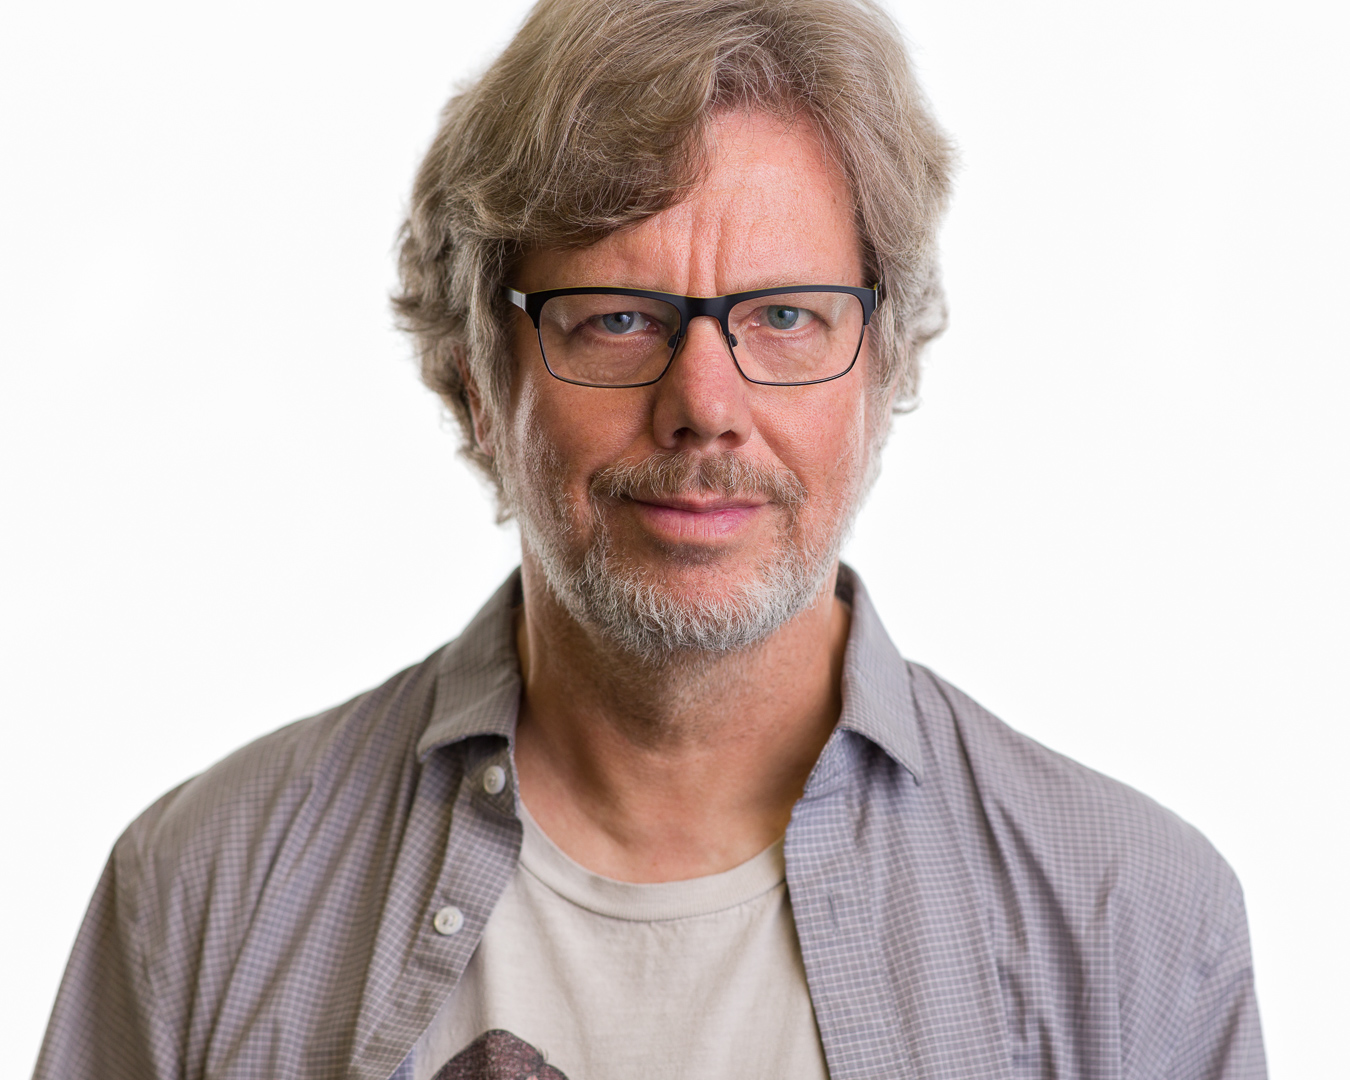
\includegraphics[width=0.25\textwidth]{pictures/guido}
\caption{Гвідо ван Россум}
\label{gvido}
\end{wrapfigure}
Python (Пайтон) — інтерпретована об'єктно-орієнтована мова програмування високого рівня зі строгою динамічною типізацією.  Назву запозичено із назви британського шоу Монті Пайтон. Розроблена в 1990 році Гвідо ван Россумом. 
\end{frame}

\begin{frame}
\frametitle{Версії Python}
%\begin{wrapfigure}{r}{0.35\textwidth}
\begin{figure}
  \begin{center}
    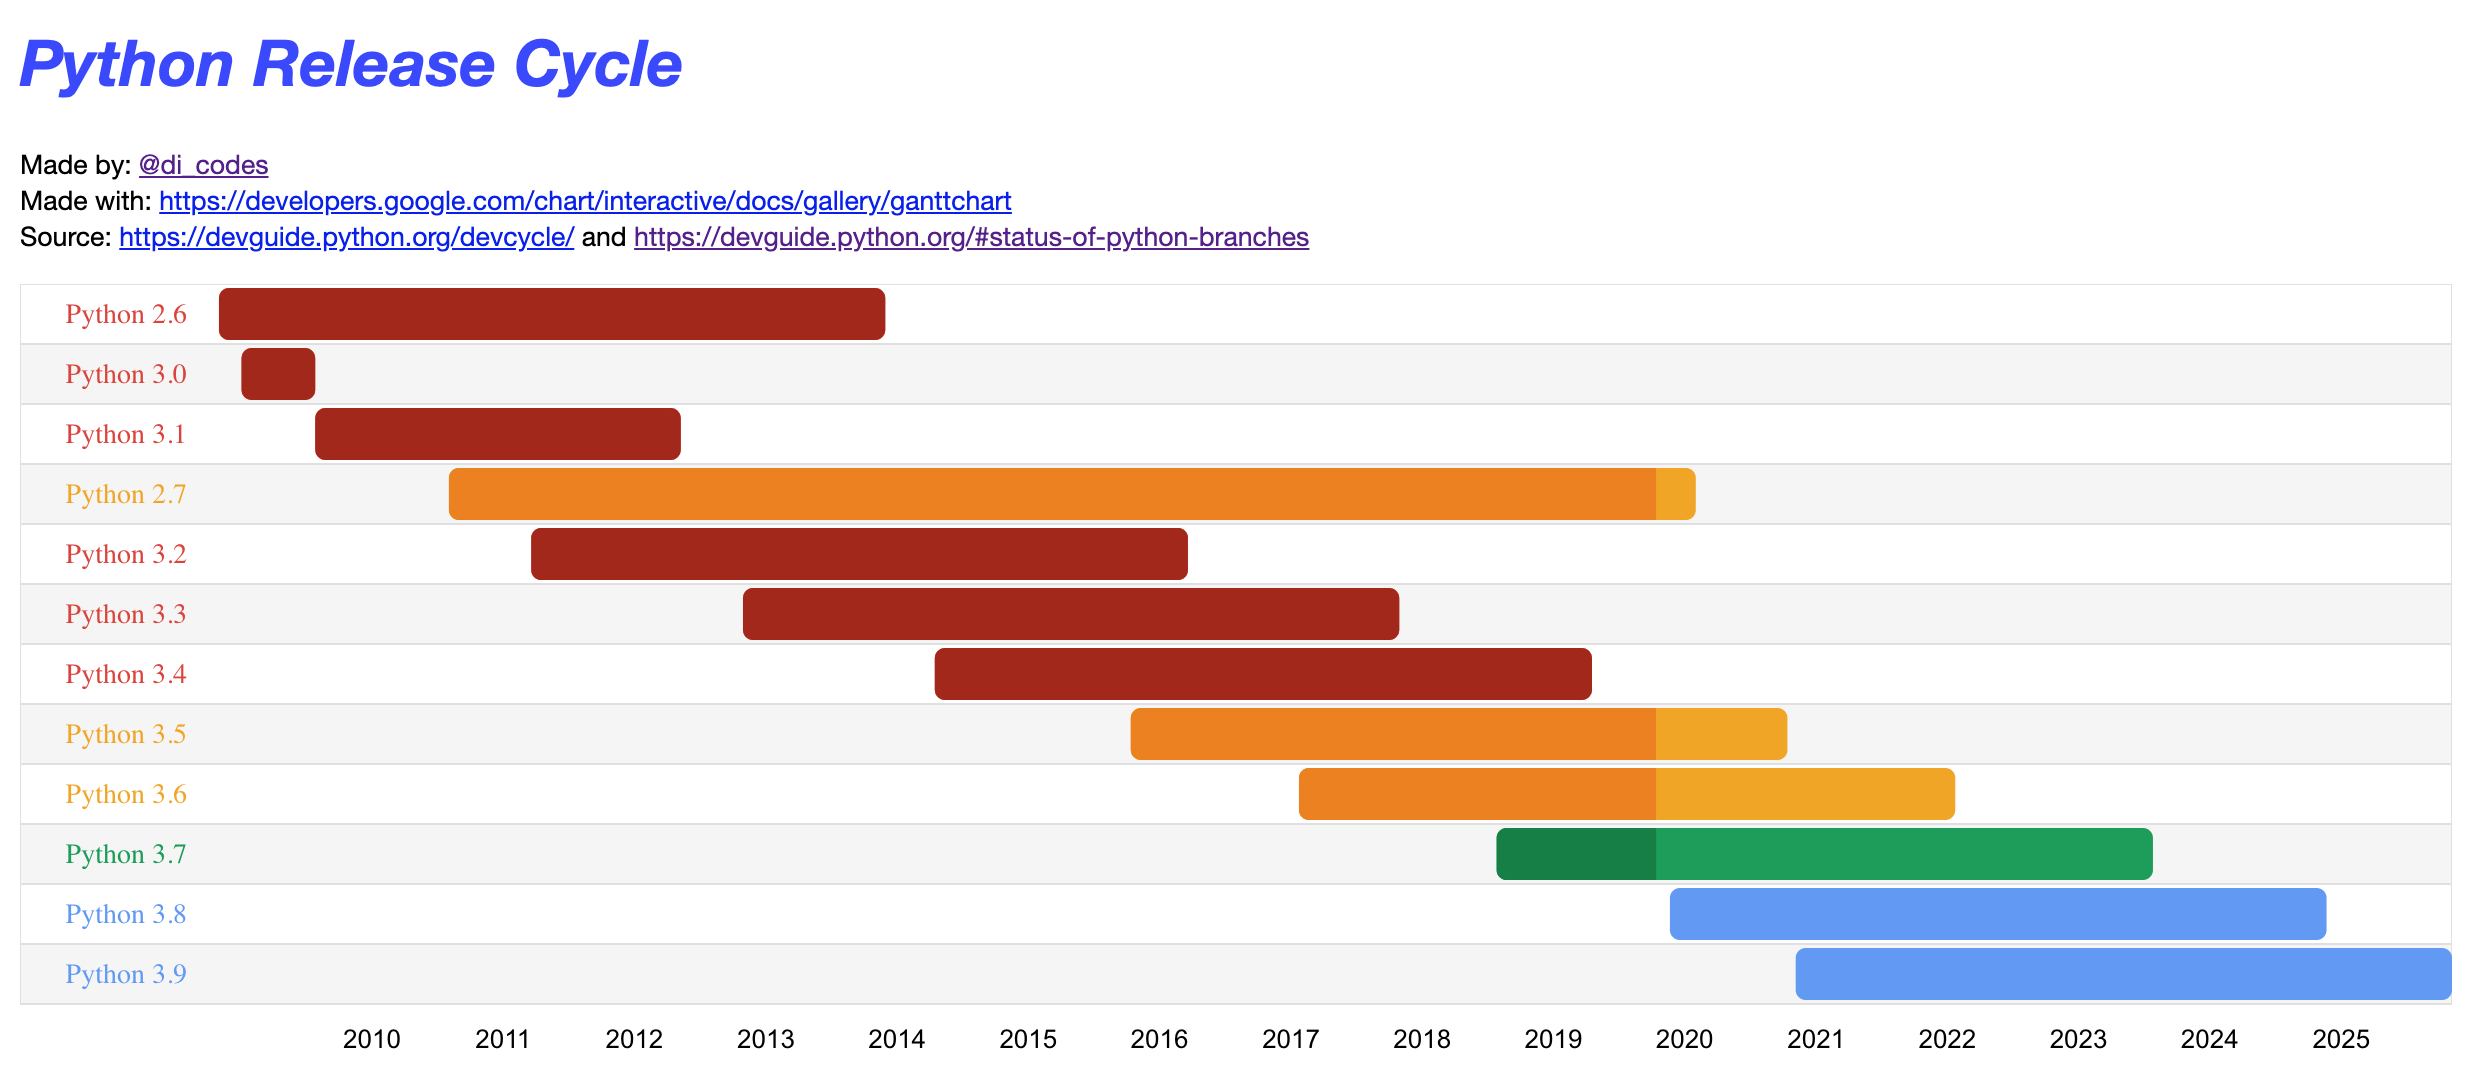
\includegraphics[width=\textwidth,height=0.5\textheight]{pictures/python_versions}
  \caption{Версії Python та період їх підтримки}
\label{versions}
  \end{center}
\end{figure}
\end{frame}

\begin{frame}
\frametitle{Переваги та недоліки Python}
Переваги:
\begin{itemize}
  \item зручність та простота програмування;
  \item переносимість програм;
  \item велика кількість модулів;
  \item поширеність та популярність.
\end{itemize}
Недоліки:
\begin{itemize}
  \item порівняно низька швидкість виконання програм;
  \item неможливість модифікації вбудованих класів.
\end{itemize}
\end{frame}

\begin{frame}
\frametitle{Переваги та недоліки Python}
\begin{itemize}
  \item Python  застосовується при розробці алгоритмів штучного інтелекту (в нейронних мережах);
  \item Python  застосовується при розробці серверної частини сайтів за допомогою Django та Flask (Instagram, YouTube, алгоритми пошуку Google, Dropbox, тощо);
  \item Python  застосовується в наукових проєктах та для обробки даних (Big Data);
  \item Python  застосовується для Web Parsing.
\end{itemize}
\end{frame}


\begin{frame}
\frametitle{Зручність та простота коду Python}
\begin{figure}
\begin{center}
 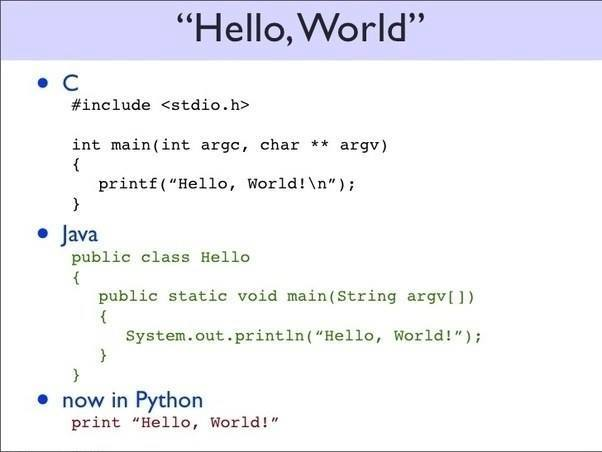
\includegraphics[width=0.4\textwidth]{pictures/helloworld.png}
\caption{Код на C, Java та Python для виведення на екран рядку "Hello, World!"}
\label{python_site} 
\end{center}
\end{figure}
\end{frame}

\begin{frame}
\frametitle{Python має велику кількість бібліотек та фреймворків}
\begin{figure}
\begin{center}
 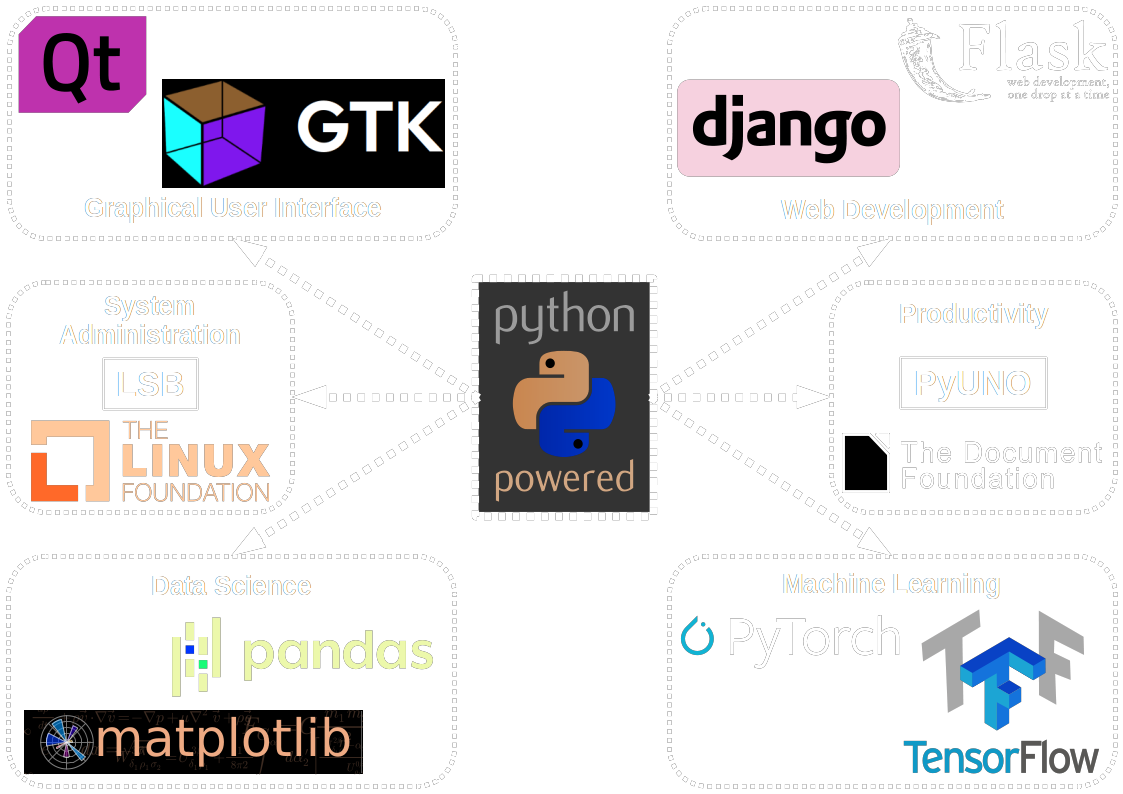
\includegraphics[width=0.6\textwidth]{pictures/python_frameworks1.png}
\caption{Фреймворки Python}
\label{python_site} 
\end{center}
\end{figure}
\end{frame}

\begin{frame}
\frametitle{Python є однією із найпопулярніших мов програмування}
\begin{figure}
\begin{center}
 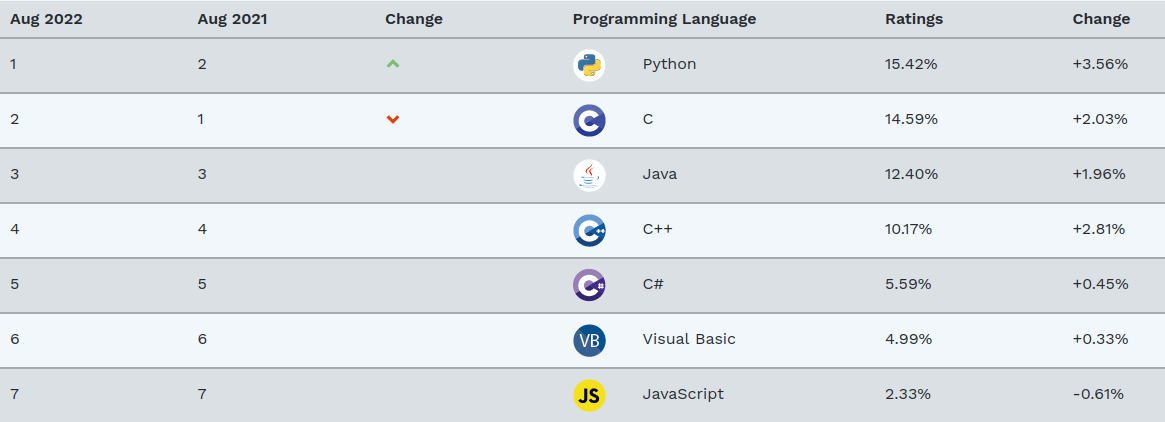
\includegraphics[width=0.6\textwidth]{pictures/tiobe.png}
\caption{З сайту \href{https://www.tiobe.com/tiobe-index/}{TIOBE}}
\label{python_site} 
\end{center}
\end{figure}
\tiny{TIOBE індекс (рейтинг мов програмування) — показник популярності мов програмування. Розраховується виходячи з кількості результів запитів до пошукових систем, що містять назву мови. Охоплює пошуки в Google, MSN, Yahoo!, Baidu, Вікіпедії і Youtube.}
\end{frame}



\subsection{Робота з Python}
\begin{frame}
\frametitle{Сайт Python}
\begin{figure}
\begin{center}
 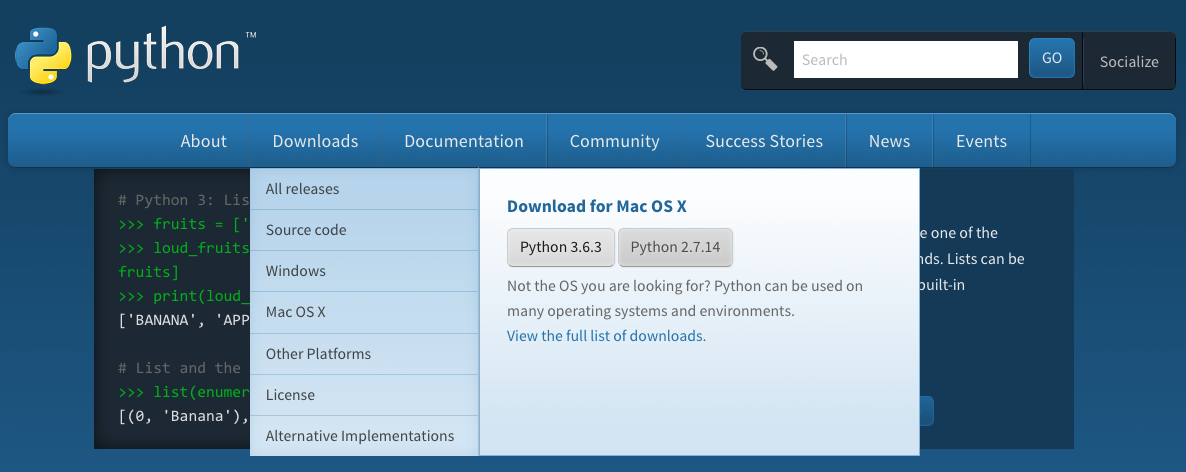
\includegraphics[width=0.95\textwidth]{pictures/python_site.png}
\caption{Сайт: \href{https://python.org/}{python.org}}
\label{python_site} 
\end{center}
\end{figure}

\end{frame}

\begin{frame}
\frametitle{Встановлення Python}
\begin{figure}
\begin{center}
 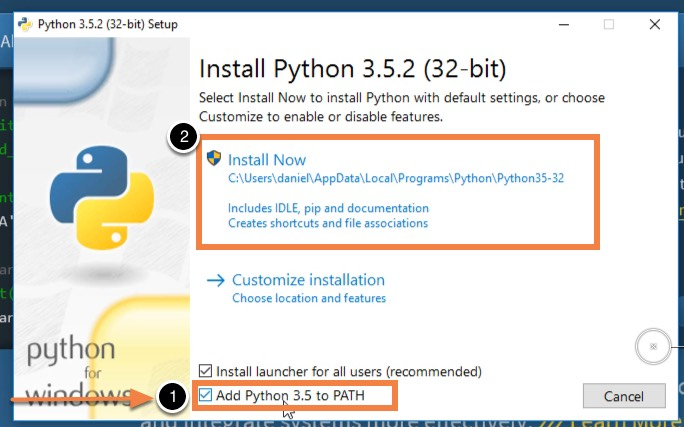
\includegraphics[width=0.4\textwidth]{pictures/python_install.jpg}
\caption{Встановлення Python}
\label{python_install} 
\end{center}
\end{figure}
\tiny{\href{https://uk.wikibooks.org/wiki/}{uk.wikibooks.org/wiki/Пориньте\_у\_Python\_3/Встановлення} - інструкція зі встановлення Python.}
\end{frame}

\begin{frame}
\frametitle{Виконання коду Python}

\begin{wrapfigure}{l}{0.45\textwidth}
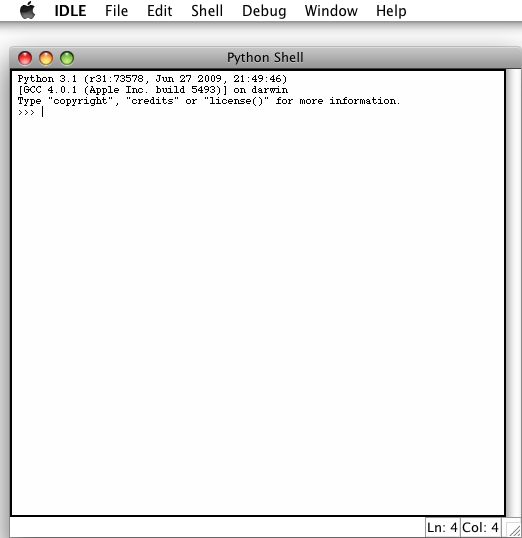
\includegraphics[width=0.35\textwidth]{pictures/idle.png}
\caption{IDLE}
\label{myphoto}
\end{wrapfigure}

Код Python може виконуватися в \textit{інтерактивному} та \textit{файловому} режимі.
\end{frame}


\begin{frame}
\frametitle{Виконання коду Python}
\href{https://it-need.com/pep-8-posibnyk-z-napysannya-kodu-na-python/}{PEP8} містить перелік принципів написання красивого та лаконічного програмного коду мовою Python (PEP – Python Enhancement Proposal, пропозиції щодо розвитку Python).
\begin{figure}
\begin{center}
 
\includegraphics[width=0.5\textwidth]{pictures/pep8.png}
\caption{PEP8}
\label{python_site} 
\end{center}
\end{figure}
\end{frame}

\begin{frame}
\frametitle{PyCharm}


\begin{wrapfigure}{r}{0.4\textwidth}

\includegraphics[width=0.25\textwidth]{pictures/pycharm_logo.png}
\caption{Логотип PyCharm}
\label{pycharm_logo}
\end{wrapfigure}

\textbf{PyCharm} — інтегроване середовище розробки для мови програмування Python. \href{https://www.jetbrains.com/pycharm/download/}{Сайт} для завантаження PyCharm.
\end{frame}


\subsection{Організація курсу}
\begin{frame}
\frametitle{Структура курсу}
\begin{itemize}
  \item 15 лекційних занять (30 годин);
  \item залікове заняття на 16 лекції (2 години);
  \item самостійна робота (58 годин).
\end{itemize}
\end{frame}

\begin{frame}
\frametitle{Нарахування балів}
\begin{itemize}
  \item Опитування за допомогою гугл-форм після кожної лекції (до 5 балів);
  \item Залікове опитування за допомогою гугл-форм на останньому занятті (до 60 балів);
  \item Додаткові бали можна отримати за представлення власних програм на Python.
\end{itemize}
\end{frame}

\begin{frame}
\frametitle{Матеріали курса}
\begin{itemize}
  \item Посилання на гугл-папку на сайті \href{http://rbecs.karazin.ua}{rbecs.karazin.ua}.
  \item Телеграм канал \href{https://t.me/python_karazin_autumn22}{t.me/python\_karazin\_autumn22}.
\end{itemize}
\end{frame}
